\section{Behaviour Driven Development}
  Beavhiour Driven Development basiert auf den Ideen von TDD und erweitert diese
  um wichtige Namenskonventionen und Begriffe, sodass klarer wird welche Schritte
  wie als Programmierer\_inn zu befolgen sind um qualitativ hochwertige Software
  zu entwicklen.\\
  Diese Erweiterung f"uhrt neue Begriffe und Werkzeuge in vier Bereichen
  \begin{itemize}
    \item Vokabular
    \item Frameworks
    \item Methodik
    \item User-Stories
  \end{itemize}
  in den TDD Zyklus ein und f"ugt einen TDD umfassenden Zyklus hinzu.

  \subsection{Unterschiede zu Test Driven Development}
    \subsubsection{Vokabular}
      ist der gr"o"ste Unterschied zu TDD. Denn bei BDD
      ist der Fokus wie der Name schon sagt auf 'Behaviour (Verhalten)' der 
      Software gelegt. Dadurch wird den Entwickler\_innen klarer deutlich
      das es in diesem Entwicklungsprozess nicht um vorzeitiges ausf"uhrliches
      White-Box-Testing einer Software geht, sondern um ein vom gew"unschten 
      Verhalten der Software getriebenes Design.\\
      In BDD wird daher nicht als erstes die Struktur des Quellcodes durch die 
      Entwickler\_innen durch Tests gepr"uft, sondern auf das gew"unschte
      Verhalten der Software von aussen eingegangen. Hierzu werden zusammen
      mit den Stakeholdern User-Stories in Form der {\em Gherkin}\cite{Gherkin} Sprache verfasst, die
      dann automatisiert in Verhaltenstest der Software umgewandelt werden.
      Dadurch ist es m"oglich das die Stakeholder schnell und einfach das 
      Verhalten gew"unschte Verhalten ihrer Software definieren k"onnen und
      die Entwickler\_innen nun gegen dieses Verhalten entwicklen.\\
      Die {\em Gherkin-Sprache} ist in einer Englisch nahen Syntax 
      gehalten und basiert im Grunde auf den drei Stichw"ortern 'Given', 'When' 
      und 'Then'. Nun wird in simplen englischen S"atzen definiert welche 
      Vorbbedingung gelten sollten ('given'), durch welche Ereignisse die 
      Nachbedingung erforderlich wird ('when') und welche Nachbedingung gelten
      sollte ('then'). Dadurch ist es nun den Stakeholdern m"oglich direkt 
      das gew"unschte Verhalten zu spezifizieren.\\
      Hier ist dies ein BDD-Feature f"ur einen einfachen Taschenrechner, welches
      nur das Verhalten f"ur Multiplikationen definiert. Wie zusehen ist, ist 
      es ohne extensive Vorkenntnisse m"oglich Features in {\em Gherkin} zu spezifizieren.
      \lstinputlisting[caption=Gherkin Beispiel ({\em Ruby} Cucumber)]{../features/multiplication.feature}
      Nat"urlich stellt sich nun die Frage wie aus diesem leicht strukturierten
      Fliesstext automatisiert Testf"alle f"urdie Entwickler\_innen erstellt werden.
      Dies l"ost {\em Cucumber}\cite{Cucumber}, ein BDD Framework f"ur {\em Ruby}, in dem die Entwickler\_innen durch Definition kleiner Regex-Schritte angebeben 
      welches Satz Schema welche Bedeutung hat.
      \lstinputlisting[caption=Schritte Definition (Cucumber),firstline=7]{../features/step_definitions/calculator_steps.rb}
      Sobald diese Definition existieren sind Stakeholder sogar in der Lage
      selbstst"andig die Testf"alle auszuf"uhren und Feedback dar"uber zu 
      erhalten wie weit es mit der Implementierung der Software fortgeschritten
      ist.\\\\

      Den wichtigsten Vorteil und Unterschied den die {\em Gherkin-Sprache} 
      mit sich bringt ist, das nun eine klar definierte kommunikation zwischen 
      Stakeholder und Entwickler\_innen m"oglich ist. Hierdurch wird die 
      Fehlerquelle des falschen Verstehens der Anforderungen durch die 
      Entwickler\_innen nahezu komplett Ausgeschaltet und sie k"onnen sich darauf
      konzentrieren das Verhalten ihrer Software an die durch die Stakeholder
      geschaffenen Verhaltenstests anzupassen.\\\\

      Ausserdem enth"alt BDD ebenfalls Tools und Empfehlungen wie Testmethoden
      zu bennen sind um aus diesen automatisch Dokumentation des Verhaltens 
      der Software zu generieren, welche auch noch von nicht Entwickler\_innen
      lesbar ist. Hierzu gibt es ja nach Tool unterschiedlich konventionen.\\
      In diesem Fall {\em RSpec}\cite{Rspec}, ein Tool was f"ur Tests in BDD 
      Prozessen und auch als alleinstehendes TDD Tool geeignet ist. Es ist aus 
      {\em RBehave}\cite{North:2007}, dem ersten BDD Tool f"ur {\em Ruby} hervorgegangen.
      \lstinputlisting[caption=RSpec Beispiel,firstline=3,lastline=14]{../spec/calculator_spec.rb}
      Wie man leicht erkennen kann ist diese Ruby DSL (Domain Specific Language)
      stark an die Bed"urfnisse von Entwickler\_innen zum schrieben von Test
      angepasst und generiert auf Anfrage automatisch folgende Dokumentation.
      \begin{lstlisting}[caption=RSpec Documentation Ausgabe]
Calculator
  addition
    should add correctly
  multiplication
    should multiply correctly
  division
    should divide correctly
      \end{lstlisting}
      Diese klar strukturierte Ausgabe bietet nat"urlich viele Vorteile gegen"uber
      der Standard Unit-Test-Suite von Ruby, welche nicht in der Lage ist 
      automatische Documentation zu generieren und keine Namenskonventionen 
      fordert.\\
      Ein weiterer Vorteil den moderne BDD Tools wie {\em RSpec } mit sich bringen
      sind speziell angepasste Methoden wie {\em it() }, {\em context()} und 
      {\em describe() }, die die Entwickler\_innen immer im Kopf behalten lassen
      das der derzeitige Fokus auf verhalten Tests liegt.

    \subsubsection{Frameworks} sind der n"achste gro"se Unterschied zu TDD. Denn 
      BDD ist nicht nur eine Art \& Weise Software zu Entwickeln, sondern verlangt
      und bietet auch das die Entwickler\_innen und Stakeholder die gleichen
      Tools verwenden um an diesem Prozess teilzunehmen.\\
      D.h. im kleinen das Stakehodler die Verhaltenstests ebenso wie 
      Entwickler\_innen in der {\em Gherkin-Sprache } spezifizieren und es 
      auf Grund von Tools wie {\em RSpec } zu jedem Test eine von Stakeholdern
      lesbare Dokumentation gibt, die automatisch aus dem Testfall generiert wird.\\
      In weiterem Sinne geh"oren hierzu auch Tools wie Git zur Versionierung, 
      Jenkins f"ur Integration Testing, Pivotal Tracker zur kolloborativen 
      Beschreibung von Bugs und Features. 

  \subsection{Workflow in Behaviour Driven Development}
    Grundlegend ist der Workflow "ahnlich zu dem bei TDD, allerdings gibt es 
    bei BDD noch einen "au"seren Zyklus, der prim"ar von Stakeholdern bestimmt wird.
    \begin{wrapfigure}{r}{0.65\textwidth}
      \vspace{-30pt}
      \begin{center}
        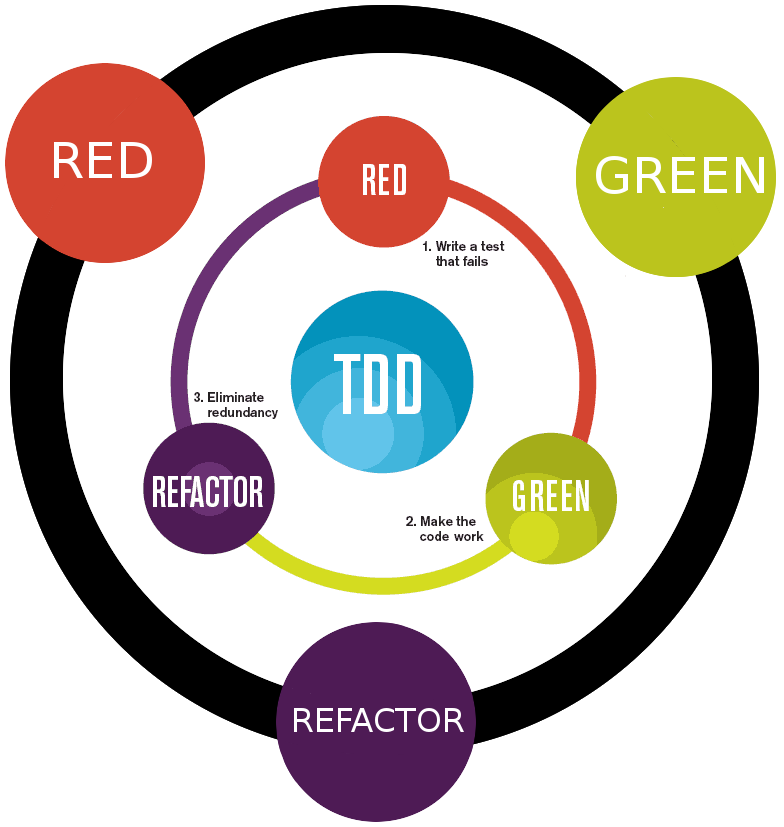
\includegraphics[scale=0.3]{assets/bdd_flow.png}
      \end{center}
      \caption{BDD-Workflow}
      \vspace{-15pt}
    \end{wrapfigure}
    Dieser "au"ser Zyklus bedeutet nichts anderes als das Stakeholder Stories
    definieren um Verhalten der Software zu spezifizieren und sie somit bestimmen
    wann alle Stories 'gr"un' sind. Die Entwickler\_innen haben nun die m"oglichkeit sich einfach Feature f"ur Feature an den Stories der Stakeholder entlang zu 
    hangel und diese nacheinander zu Implementieren. Dabei werden bis auf die 
    zeitliche L"ange eines Features die gleichen Massgaben wie bei TDD beachtet.\\
    Der innere Zyklus kommt nur zustande, falls die Features definierten Features
    von den Stakeholdern komplexer gew"ahlt sind. Dann k"onnen die Entwickler 
    diese nach TDD Prinzipien entwickeln und somit am Schluss sicher seien 
    dass ihr entwickeltes Feature minimal ist und trotzdem das gew"unschte 
    Verhalten repr"asentiert.\\

  \subsection{Beispiel: Umsetzung mit Cucumber/Rspec in Ruby}
    Am Beispiel einer Taschenrechner-Klasse in Ruby wollen wir nun die 
    Unterschiede zwischen Behaviour Driven Development und Test Driven 
    Development nachvollziehen.
    \subsubsection{TDD:}
      In TDD w"urden wir als erstes diese folgenden Tests spezifizieren 
      und dann die gew"unschten Features implementieren.
      \lstinputlisting[caption=Ruby UnitTest,firstline=5]{../tests/calculator_test.rb}

    \subsubsection{BDD:}
      In BDD hingegen w"urden wir als erstes Stories f"ur das gew"unschte
      Verhalten schreiben und f"ur diese dann auch die passenden Step-Definitionen
      wie in Listing 1.1 und 1.2 gezeigt.\\
      Danach w"urden wir die gew"unschten Features implementieren und diese
      fals es die komplexit"at verlangt nochmal einzeln in TDD entwickeln.\\
      Die genutzte Toolchain w"are Cucumber f"ur BDD und RSpec f"ur TDD.

  \subsection{Anderere Sprachen, andere Tools}
    Falls BDD in anderen Sprachen verfolgt werden soll gibt es hier eine nicht
    vollst"andige Liste mit anderen g"angigen Tools:
    \begin{itemize}
      \item Java -> \href{http://http://jbehave.org/}{JBehave}
      \item C -> \href{http://code.google.com/p/cbehave/}{CBehave}
      \item Ruby -> \href{http://cukes.info}{Cucumber}, \href{http://rspec.info}{RSpec}
      \item PHP -> \href{http://behat.org}{behat}
      \item Python -> \href{http://lettuce.it}{Lettuce}
    \end{itemize}